\section{Simulation Analysis}
\label{simuanal}

In order to understand the values obtained in our simulation, it is important to note a couple of things:
\begin{itemize}
    \item Node 4 is considered to be ground, therefore, its' voltage is not shown in the table of results, but is, obviously, 0V.
    \item To compute the voltage drop through the dependent voltage source ($V_d$), we needed to obtain
the current value through resistor R6. However, Ngspice doesn’t allow us to input Resistor $R_6$ current in the computation. Hence, in order to solve this problem, we introduced a voltage source
with no voltage drop in series with the $R_6$ resistor. This way, we managed to obtain the current
through it, and therefore we were able to compute the dependent voltage source $V_d$.
\end{itemize}

\subsection{Circuit Analysis for $t \leq 0 $}

For $t < 0$, the voltage source (Va) is producing a constant voltage source of value Vs. Therefore, the capacitor behaves as an open circuit. After running the Ngspice script, we obtained the following results:

\begin{table}[h]
\centering
\begin{tabularx}{0.6\textwidth} {
  | >{\raggedright\arraybackslash}X
  | >{\raggedleft\arraybackslash}X | }
 \hline
@gb[i] & -2.39986e-04\\ \hline
@r1[i] & -2.29300e-04\\ \hline
@r2[i] & -2.39986e-04\\ \hline
@r3[i] & -1.06863e-05\\ \hline
@r4[i] & 1.176882e-03\\ \hline
@r5[i] & -2.39986e-04\\ \hline
@r6[i] & 9.475819e-04\\ \hline
@r7[i] & 9.475819e-04\\ \hline
v(1) & 5.114229e+00\\ \hline
v(2) & 4.873694e+00\\ \hline
v(3) & 4.380386e+00\\ \hline
v(5) & 4.906396e+00\\ \hline
v(6) & 5.644101e+00\\ \hline
v(7) & -1.93573e+00\\ \hline
v(8) & -2.91891e+00\\ \hline
v(9) & -1.93573e+00\\ \hline

\end{tabularx}
\caption{Nodal Voltage Simulation Results. Variables expressed in V or A}
\end{table}

\begin{table}[h]
\centering
\begin{tabularx}{0.6\textwidth} {
  | >{\raggedright\arraybackslash}X
  | >{\raggedleft\arraybackslash}X | }
 \hline
V1 & 5.114229e+00 V\\ \hline
V2 & 4.873694e+00 V\\ \hline
V3 & 4.380386e+00 V\\ \hline
V4 & 0.000000e+00 V\\ \hline
V5 & 4.906396e+00 V\\ \hline
V6 & 5.644102e+00 V\\ \hline
V7 & -1.935730e+00 V\\ \hline
V8 & -2.918905e+00 V\\ \hline

\end{tabularx}
\caption{Theoretical Nodal Voltages expressed in V}
\end{table}

\begin{table}[h]
\centering
\begin{tabularx}{0.6\textwidth} {
  | >{\raggedright\arraybackslash}X
  | >{\raggedleft\arraybackslash}X | }
 \hline
I1 & -2.293000e-04 A\\ \hline
I2 & -2.399863e-04 A\\ \hline
I3 & -1.068631e-05 A\\ \hline
I4 & 1.176882e-03 A\\ \hline
I5 & -2.399863e-04 A\\ \hline
I6 & 9.475818e-04 A\\ \hline
I7 & 9.475818e-04 A\\ \hline
Is & -2.293000e-04 A\\ \hline
Ic & 0.000000e+00 A\\ \hline

\end{tabularx}
\caption{Theoretical Nodal Voltages expressed in A}
\end{table}

\subsection{$R_{eq}$ Calculus, and Circuit Analysis for $t=0$}

In the second simulation, the open circuit branch of the capacitor was replaced with a voltage source, with voltage $V_x=V_6-V_8$. This step was needed to calculate the equivalent Thévenin resistance, which can be obtained through the following expression:
\begin{equation}
     R_{eq}=\frac{V_6-V_8}{I_x}
\end{equation}


with $I_x$ being the current through the voltage source previously defined $V_x$.

\begin{table}[h]
\centering
\begin{tabularx}{0.6\textwidth} {
  | >{\raggedright\arraybackslash}X
  | >{\raggedleft\arraybackslash}X | }
 \hline
@gb[i] & 0.000000e+00\\ \hline
@r1[i] & 0.000000e+00\\ \hline
@r2[i] & 0.000000e+00\\ \hline
@r3[i] & 0.000000e+00\\ \hline
@r4[i] & 0.000000e+00\\ \hline
@r5[i] & -2.78567e-03\\ \hline
@r6[i] & 0.000000e+00\\ \hline
@r7[i] & 0.000000e+00\\ \hline
v(1) & 0.000000e+00\\ \hline
v(2) & 0.000000e+00\\ \hline
v(3) & 0.000000e+00\\ \hline
v(5) & 0.000000e+00\\ \hline
v(6) & 8.563007e+00\\ \hline
v(7) & 0.000000e+00\\ \hline
v(8) & 0.000000e+00\\ \hline
v(9) & 0.000000e+00\\ \hline

\end{tabularx}
\caption{Nodal Voltage Simulation results. Variables expressed in V}
\end{table}

\begin{table}[h]
\centering
\begin{tabularx}{0.6\textwidth} {
  | >{\raggedright\arraybackslash}X
  | >{\raggedleft\arraybackslash}X | }
 \hline
V1 & 0.000000e+00 V\\ \hline
V2 & 0.000000e+00 V\\ \hline
V3 & 0.000000e+00 V\\ \hline
V4 & 0.000000e+00 V\\ \hline
V5 & -5.941780e-17 V\\ \hline
V6 & 8.563007e+00 V\\ \hline
V7 & 0.000000e+00 V\\ \hline
V8 & 2.970890e-17 V\\ \hline
Ix & -2.785669e-03 A\\ \hline
Req & 3.073950e+03 Ohm\\ \hline
tau & 3.109455e-03 \\ \hline

\end{tabularx}
\caption{Theoretical results expressed in V, A and Ohm}
\end{table}

\subsection{Circuit Analysis for $t \geq 0 $ (Natural Solution)}

For the third simulation, we performed a transient analysis of the given circuit, which is similar to the one done in the previous section. The main difference is the introduction of the capacitor instead of the voltage source between nodes 6 and 8, and the fact that the voltage source is turned off. With this, we run the Ngspice script to obtain the natural solution of the circuit.

\begin{figure}[h] \centering
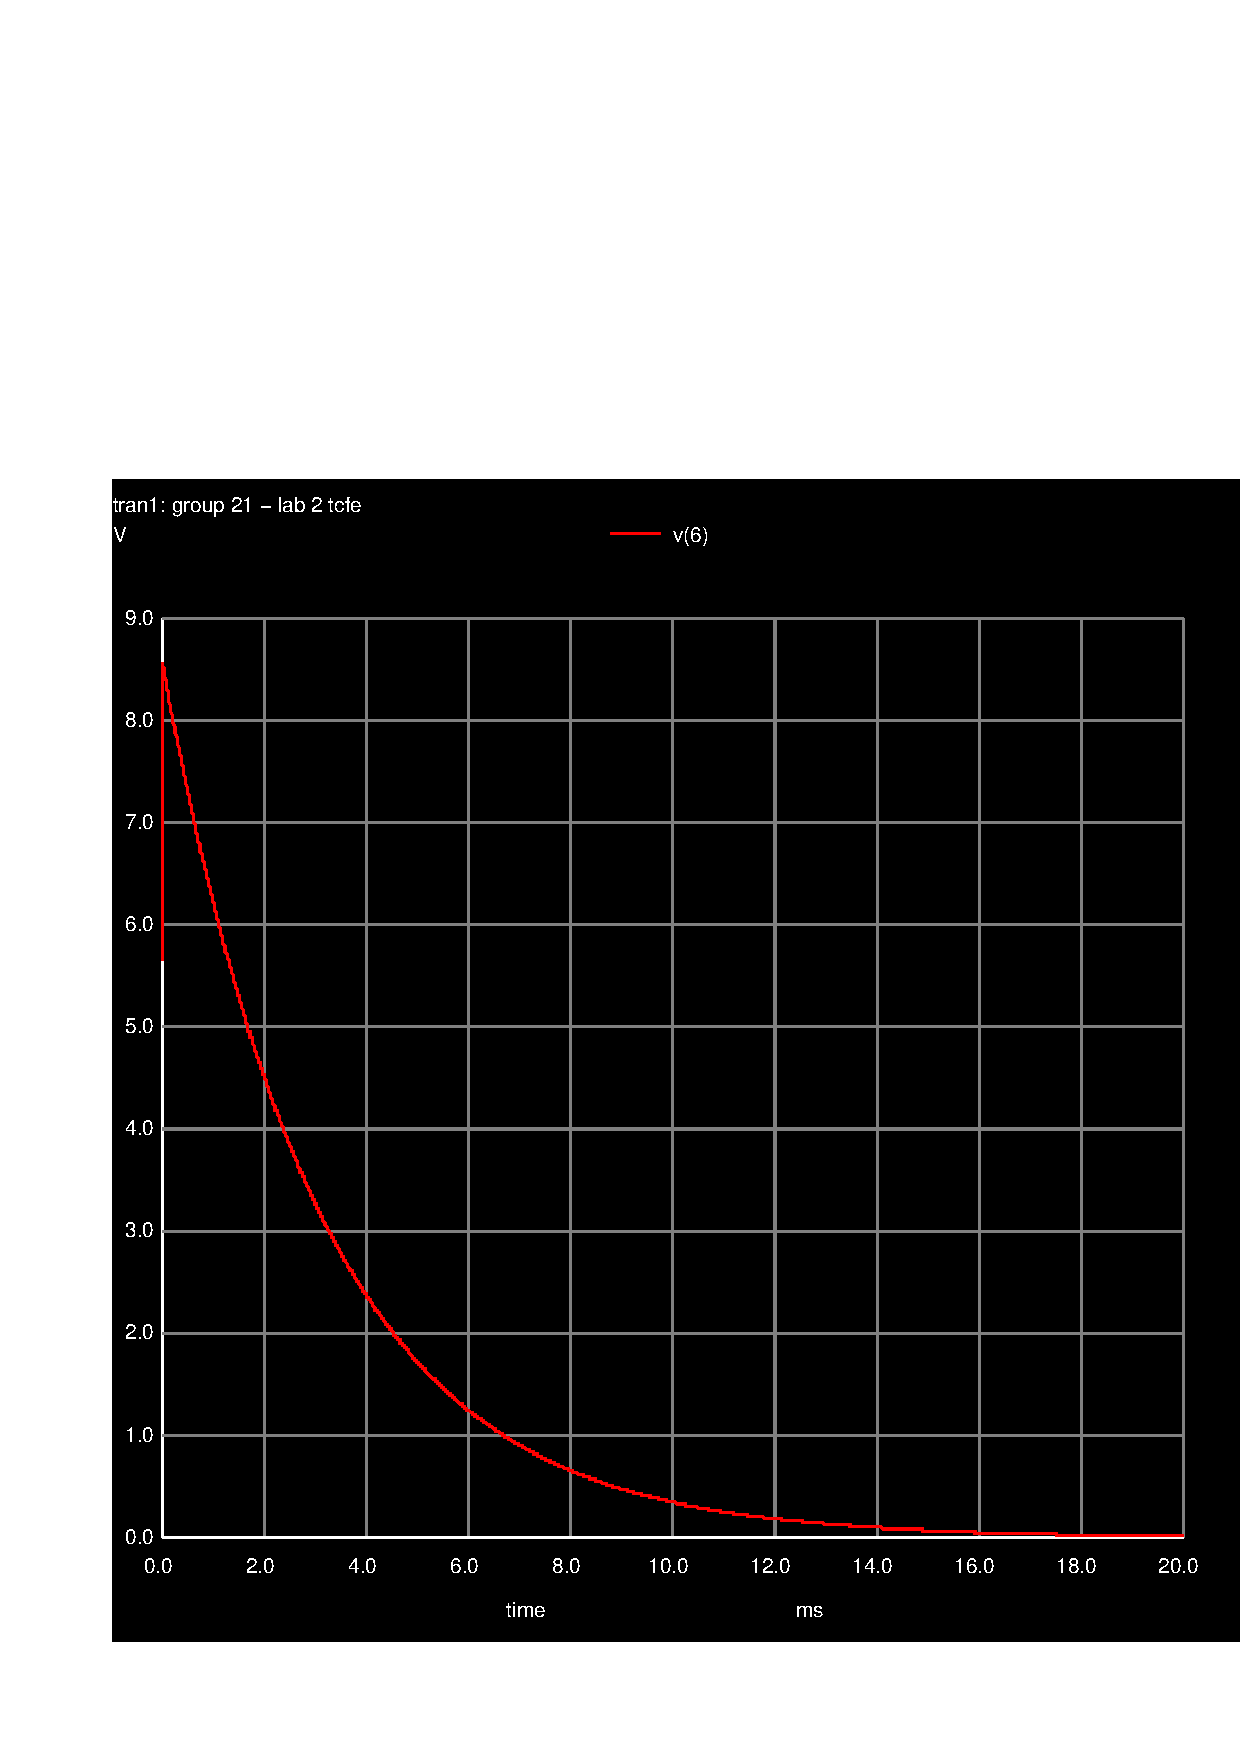
\includegraphics[width=0.7\linewidth]{question_3.pdf}
\caption{Natural Solution (Ngspice)}
\label{fig:snat}
\end{figure}

\begin{figure}[h] \centering
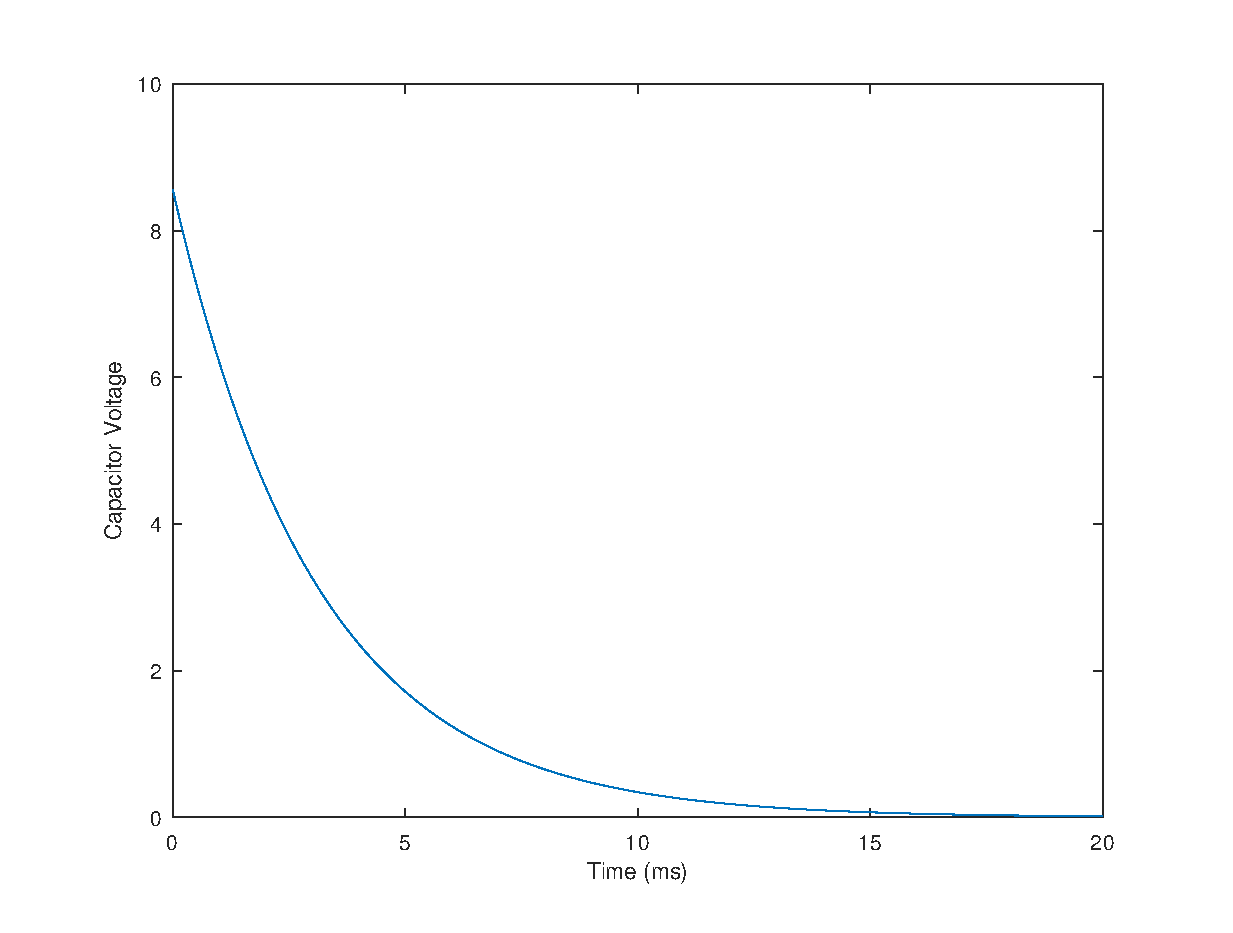
\includegraphics[width=0.7\linewidth]{naturalsolution.eps}
\caption{Natural Solution (Octave)}
\label{fig:snat}
\end{figure}


We can conclude that the capacitor is discharging over time, as expected, concluding that the theoretical analysis and the simulation, match.

\subsection{Circuit Analysis for $t \geq 0 $ (Natural and Forced Solution)}

In this section we also performed a transient analysis, making a few changes to the circuit, in order to obtain a plot of the natural and forced solution. Therefore, we took in consideration the sinusoidal variation of the voltage source over time, plotting that in our computation.

\begin{figure}[h] \centering
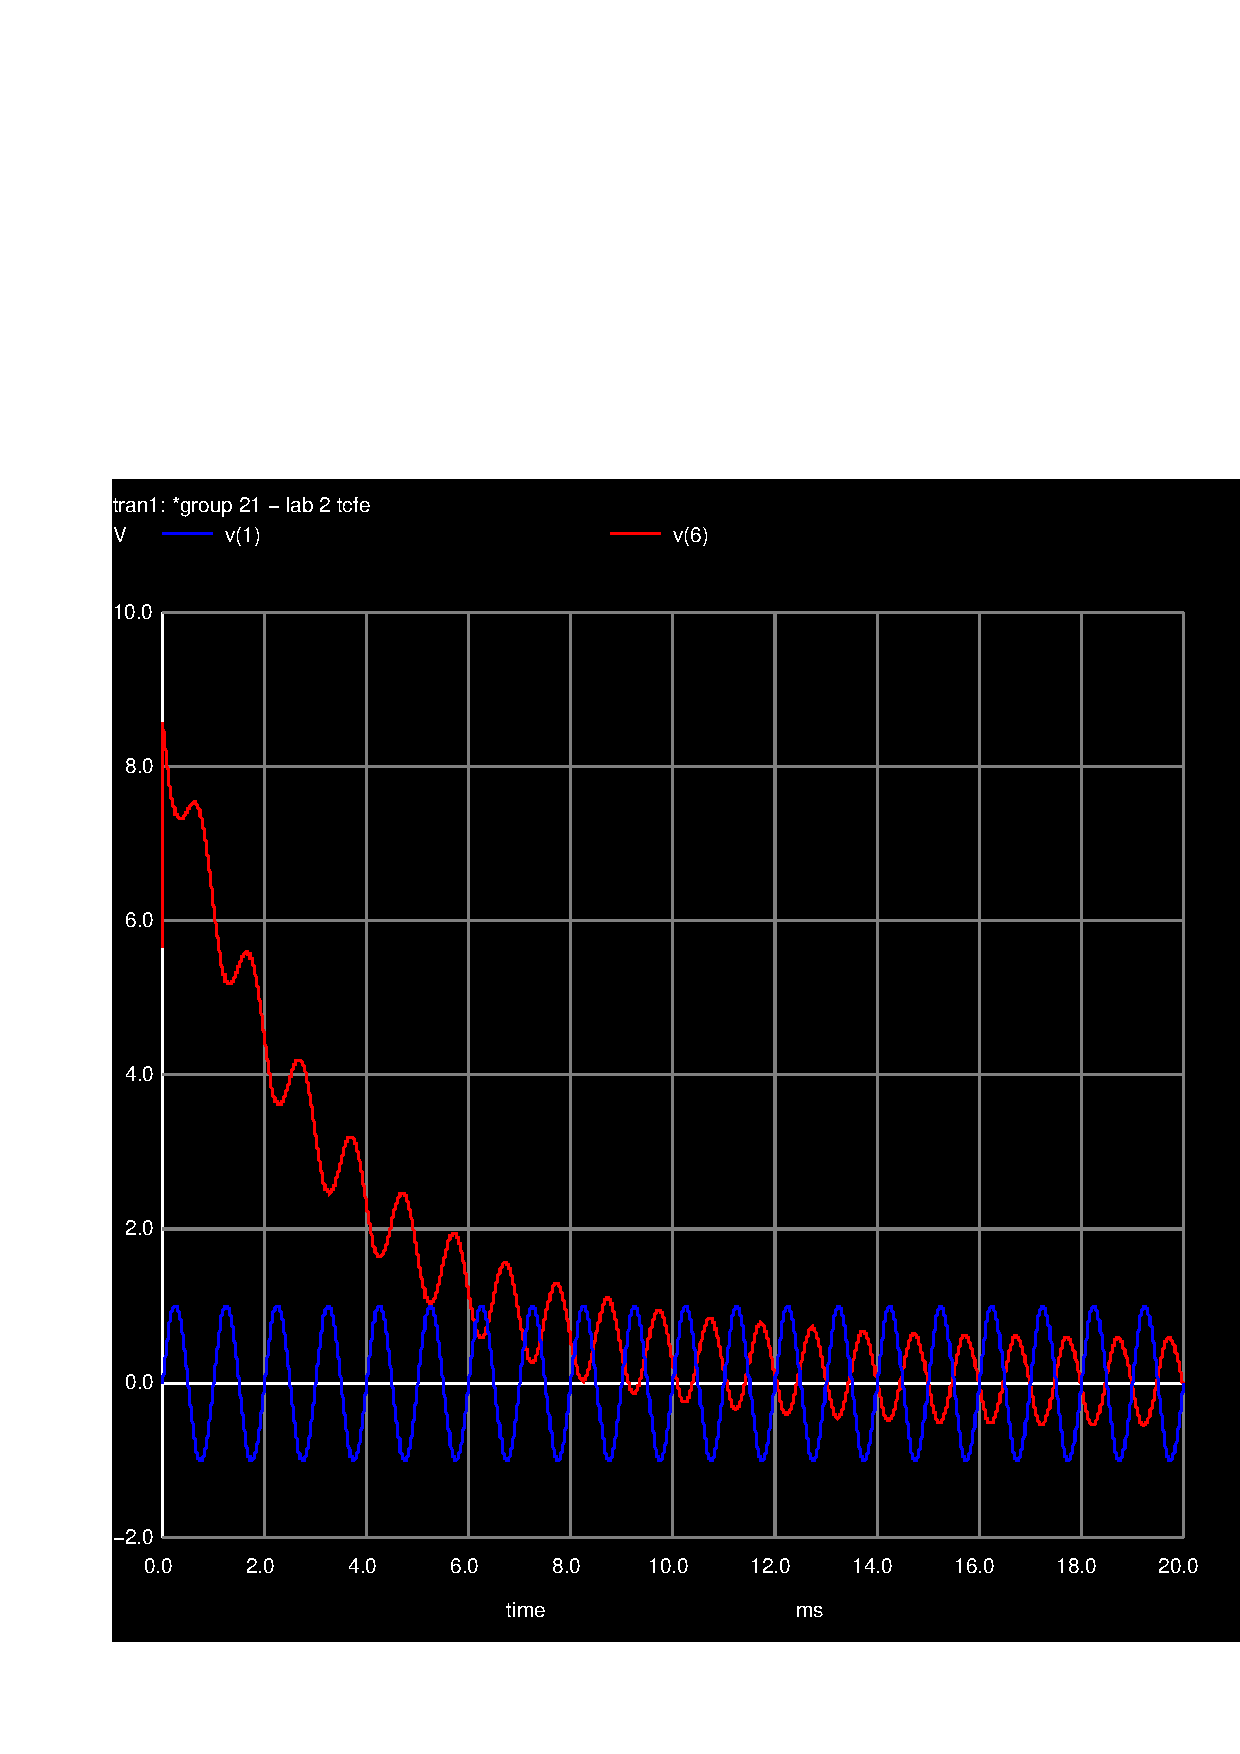
\includegraphics[width=0.7\linewidth]{question_4.pdf}
\caption{Final Solution (NGSpice)}
\label{fig:snat}
\end{figure}

\begin{figure}[h] \centering
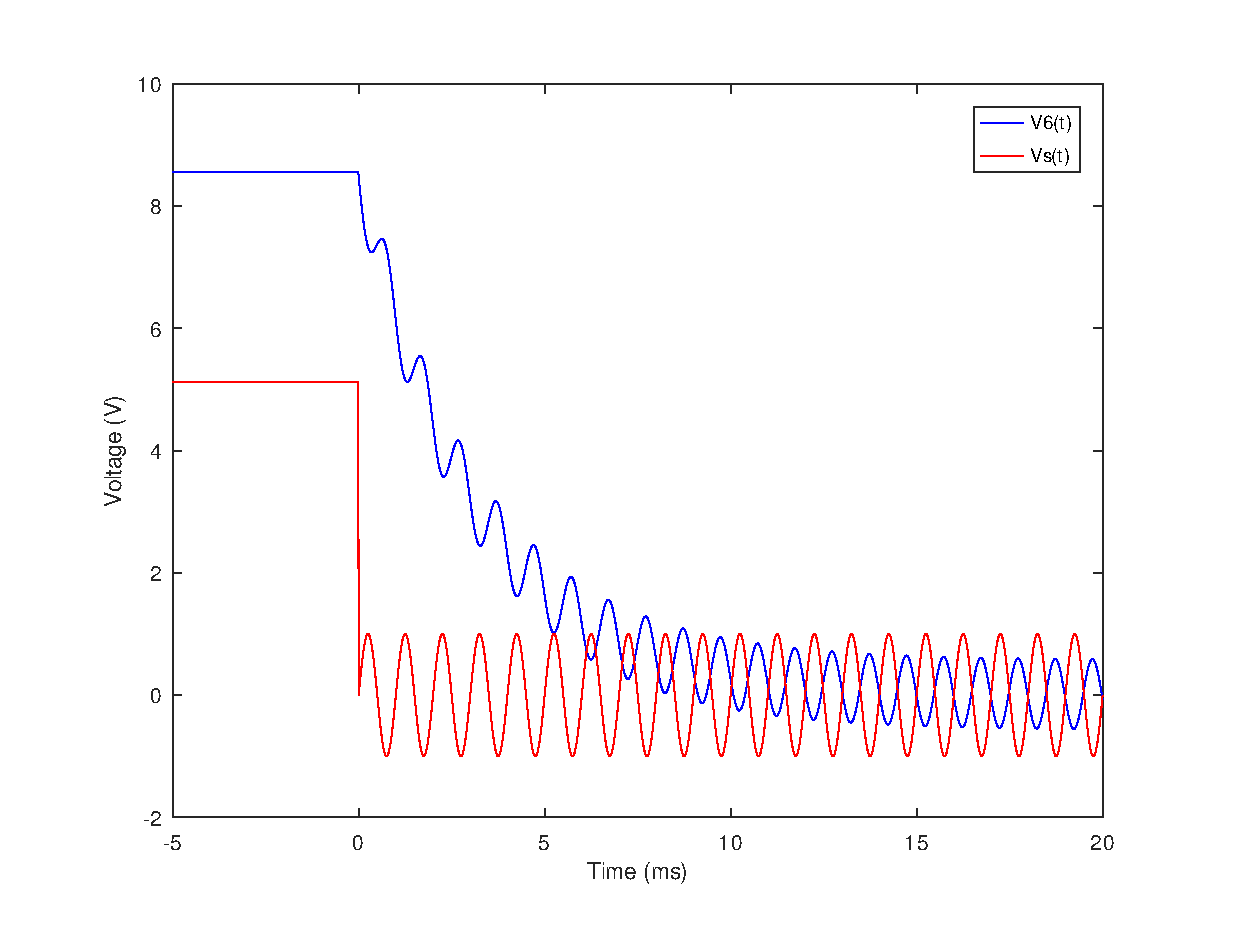
\includegraphics[width=0.7\linewidth]{forced_and_natural_solution.eps}
\caption{Final Solution (Octave)}
\label{fig:snat}
\end{figure}

As we can see from the pictures above, both Octave and Ngspice results match perfectly. W can conclude that the voltage in the capacitor diminishes until it has a phase difference of $\pi$, in comparison to the voltage source, as expected in the theoretical analysis.

\subsection{Frequency Responses}

For this section, we conducted and Alternating Current (AC) Analysis. With this, we were able to study the frequency response of the circuit. It is important to note that there is no frequency variation, which means we are performing a steady-state analysis. After examination of the graphics below, it is clear that the results from Octave match the ones of Ngspice clear, where any minor difference may be explained by approximation errors.

\subsubsection{Frequency Responses - Amplitude}

\begin{figure}
\centering
\begin{minipage}{.5\textwidth}
  \centering
  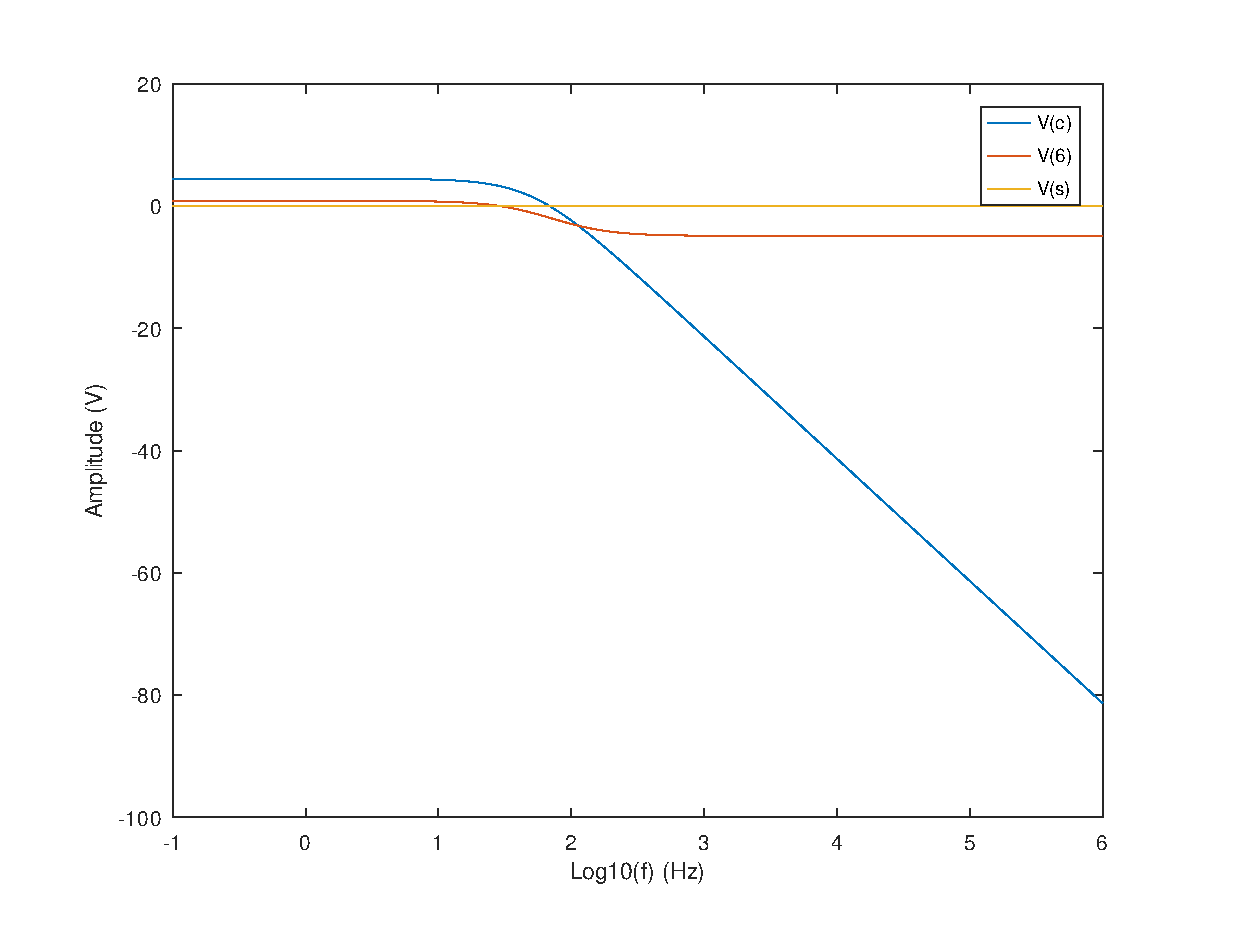
\includegraphics[width=.4\linewidth]{amplitude.eps}
  \captionof{figure}{A figure}
  \label{fig:test1}
\end{minipage}%
\begin{minipage}{.5\textwidth}
  \centering
  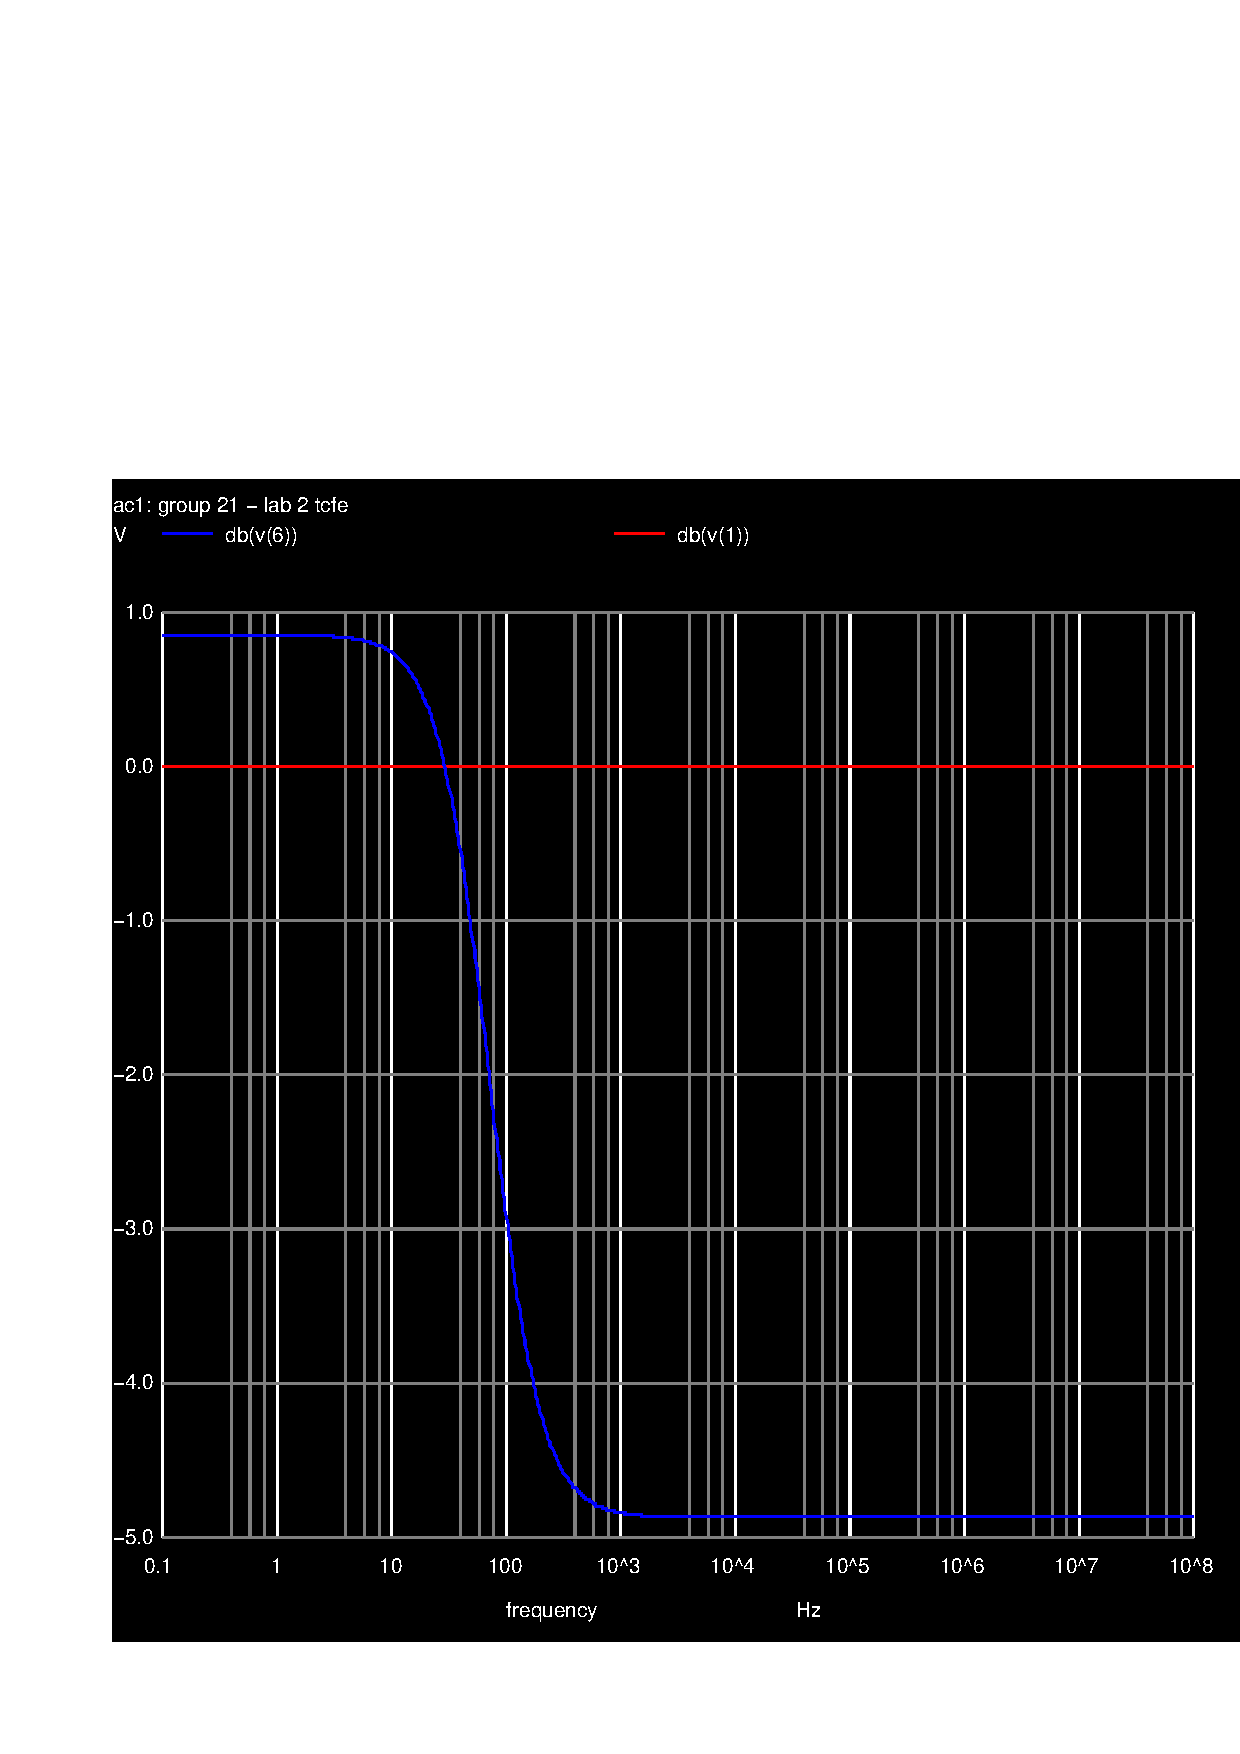
\includegraphics[width=.4\linewidth]{question5_db.pdf}
  \captionof{figure}{Another figure}
  \label{fig:test2}
\end{minipage}
\end{figure}


\subsubsection{Frequency Responses - Phase}

\begin{figure}
\centering
\begin{minipage}{.5\textwidth}
  \centering
  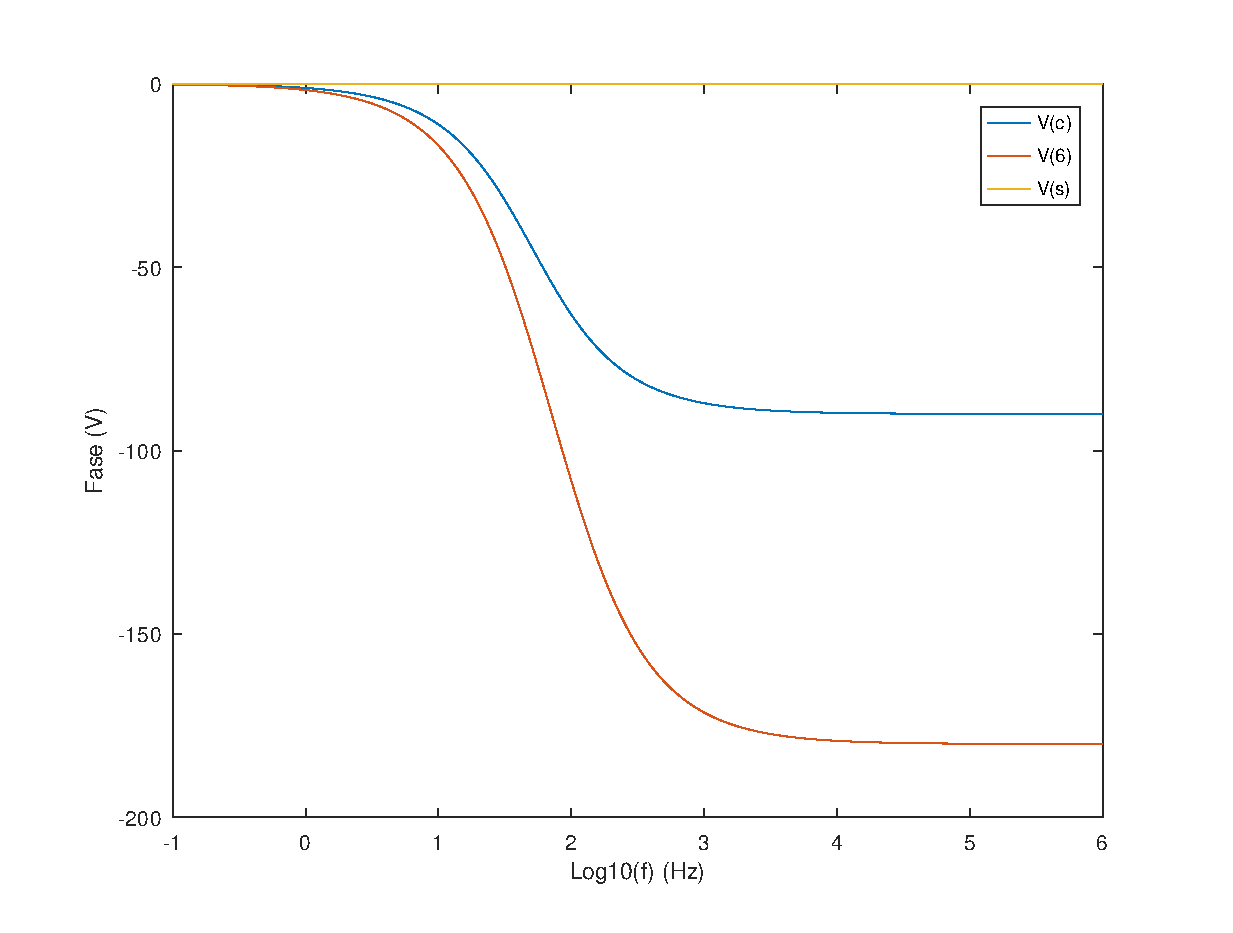
\includegraphics[width=.4\linewidth]{phase.eps}
  \captionof{figure}{A figure}
  \label{fig:test1}
\end{minipage}%
\begin{minipage}{.5\textwidth}
  \centering
  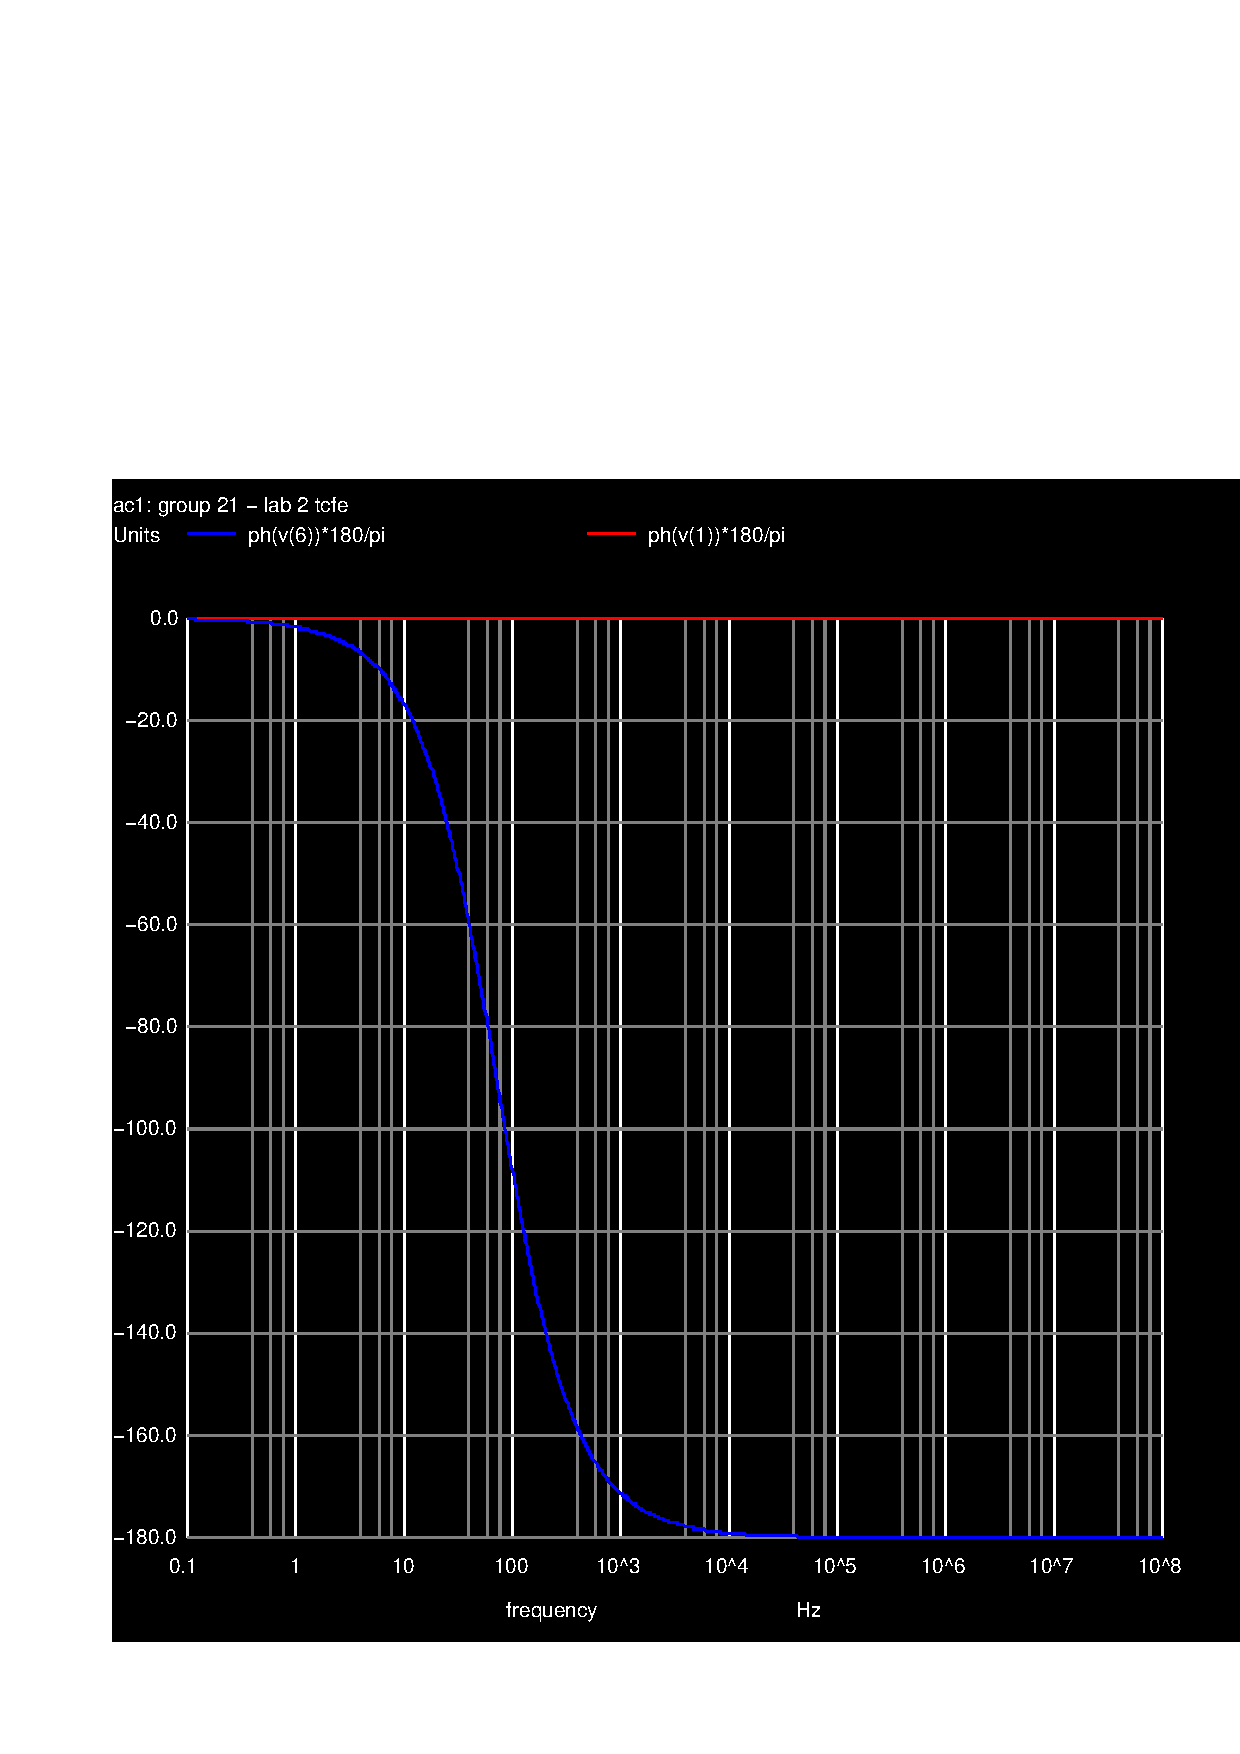
\includegraphics[width=.4\linewidth]{question5_ph.pdf}
  \captionof{figure}{Another figure}
  \label{fig:test2}
\end{minipage}
\end{figure}
